\documentclass[14pt]{extbook}
\usepackage{multicol, enumerate, enumitem, hyperref, color, soul, setspace, parskip, fancyhdr} %General Packages
\usepackage{amssymb, amsthm, amsmath, latexsym, units, mathtools} %Math Packages
\everymath{\displaystyle} %All math in Display Style
% Packages with additional options
\usepackage[headsep=0.5cm,headheight=12pt, left=1 in,right= 1 in,top= 1 in,bottom= 1 in]{geometry}
\usepackage[usenames,dvipsnames]{xcolor}
\usepackage{dashrule}  % Package to use the command below to create lines between items
\newcommand{\litem}[1]{\item#1\hspace*{-1cm}\rule{\textwidth}{0.4pt}}
\pagestyle{fancy}
\lhead{Module4}
\chead{}
\rhead{Version B}
\lfoot{2958-5637}
\cfoot{}
\rfoot{test}
\begin{document}

\begin{enumerate}
\litem{
Graph the equation below.\[ f(x) = (x+2)^2 - 18 \]\begin{enumerate}[label=\Alph*.]
\begin{multicols}{2}\item 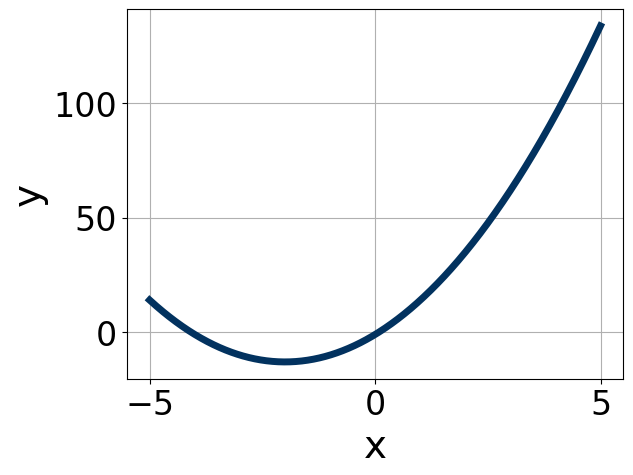
\includegraphics[width = 0.3\textwidth]{../Figures/quadraticEquationToGraphCopyAB.png}\item 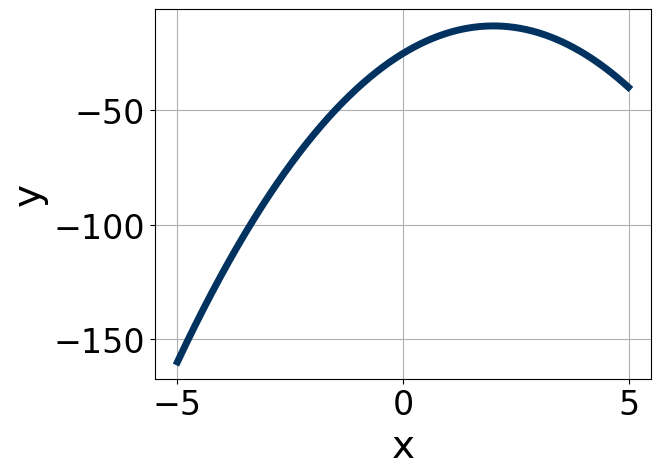
\includegraphics[width = 0.3\textwidth]{../Figures/quadraticEquationToGraphCopyBB.png}\item 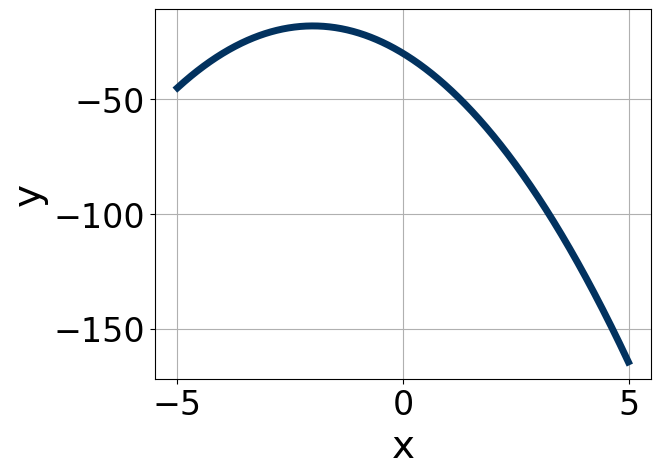
\includegraphics[width = 0.3\textwidth]{../Figures/quadraticEquationToGraphCopyCB.png}\item 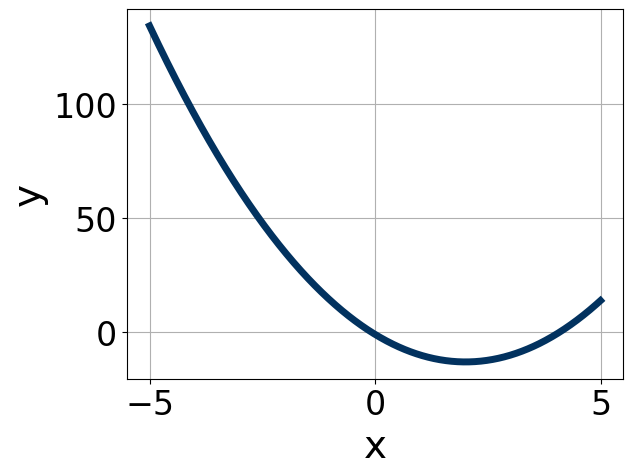
\includegraphics[width = 0.3\textwidth]{../Figures/quadraticEquationToGraphCopyDB.png}\end{multicols}\item None of the above.
\end{enumerate} }
\litem{
Factor the quadratic below. Then, choose the intervals that contain the constants in the form $(ax+b)(cx+d); b \leq d.$\[ 24x^{2} +10 x -25 \]\begin{enumerate}[label=\Alph*.]
\item \( a \in [5, 8.6], \hspace*{5mm} b \in [-9, -2], \hspace*{5mm} c \in [3.19, 4.96], \text{ and } \hspace*{5mm} d \in [1, 6] \)
\item \( a \in [11.2, 12.7], \hspace*{5mm} b \in [-9, -2], \hspace*{5mm} c \in [1.41, 2.41], \text{ and } \hspace*{5mm} d \in [1, 6] \)
\item \( a \in [-0.6, 1.6], \hspace*{5mm} b \in [-20, -14], \hspace*{5mm} c \in [-0.12, 1.91], \text{ and } \hspace*{5mm} d \in [28, 33] \)
\item \( a \in [2.8, 5.9], \hspace*{5mm} b \in [-9, -2], \hspace*{5mm} c \in [6.82, 8.5], \text{ and } \hspace*{5mm} d \in [1, 6] \)
\item \( \text{None of the above.} \)

\end{enumerate} }
\litem{
Solve the quadratic equation below. Then, choose the intervals that the solutions belong to, with $x_1 \leq x_2$ (if they exist).\[ 11x^{2} -9 x -9 = 0 \]\begin{enumerate}[label=\Alph*.]
\item \( x_1 \in [-1.8, -1.15] \text{ and } x_2 \in [0.4, 1.1] \)
\item \( x_1 \in [-6.53, -5.56] \text{ and } x_2 \in [14.6, 16.8] \)
\item \( x_1 \in [-0.82, -0.28] \text{ and } x_2 \in [0.8, 2.5] \)
\item \( x_1 \in [-22.01, -21.25] \text{ and } x_2 \in [21.4, 23.1] \)
\item \( \text{There are no Real solutions.} \)

\end{enumerate} }
\litem{
Write the equation of the graph presented below in the form $f(x)=ax^2+bx+c$, assuming  $a=1$ or $a=-1$. Then, choose the intervals that $a, b,$ and $c$ belong to.
\begin{center}
    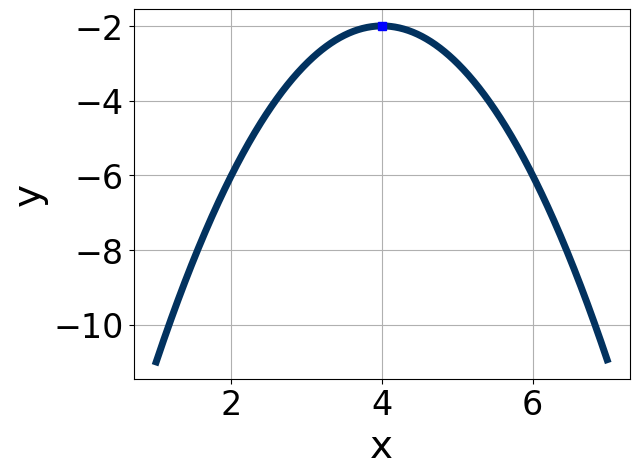
\includegraphics[width=0.5\textwidth]{../Figures/quadraticGraphToEquationB.png}
\end{center}
\begin{enumerate}[label=\Alph*.]
\item \( a \in [-1.6, -0.5], \hspace*{5mm} b \in [-11, -7], \text{ and } \hspace*{5mm} c \in [-15, -10] \)
\item \( a \in [0.1, 2.2], \hspace*{5mm} b \in [-11, -7], \text{ and } \hspace*{5mm} c \in [13, 18] \)
\item \( a \in [-1.6, -0.5], \hspace*{5mm} b \in [8, 12], \text{ and } \hspace*{5mm} c \in [-18, -15] \)
\item \( a \in [-1.6, -0.5], \hspace*{5mm} b \in [-11, -7], \text{ and } \hspace*{5mm} c \in [-18, -15] \)
\item \( a \in [0.1, 2.2], \hspace*{5mm} b \in [8, 12], \text{ and } \hspace*{5mm} c \in [13, 18] \)

\end{enumerate} }
\litem{
Solve the quadratic equation below. Then, choose the intervals that the solutions belong to, with $x_1 \leq x_2$ (if they exist).\[ -17x^{2} -12 x + 7 = 0 \]\begin{enumerate}[label=\Alph*.]
\item \( x_1 \in [-0.5, 0.1] \text{ and } x_2 \in [0.73, 1.12] \)
\item \( x_1 \in [-7.8, -5] \text{ and } x_2 \in [18.27, 18.8] \)
\item \( x_1 \in [-1.8, -0.8] \text{ and } x_2 \in [0.06, 0.91] \)
\item \( x_1 \in [-25.7, -23.9] \text{ and } x_2 \in [24.24, 25.11] \)
\item \( \text{There are no Real solutions.} \)

\end{enumerate} }
\litem{
Solve the quadratic equation below. Then, choose the intervals that the solutions $x_1$ and $x_2$ belong to, with $x_1 \leq x_2$.\[ 20x^{2} +69 x + 54 = 0 \]\begin{enumerate}[label=\Alph*.]
\item \( x_1 \in [-7.11, -6.72] \text{ and } x_2 \in [-0.46, -0.39] \)
\item \( x_1 \in [-47, -43.01] \text{ and } x_2 \in [-24.04, -23.96] \)
\item \( x_1 \in [-3.03, -1.46] \text{ and } x_2 \in [-1.32, -1.16] \)
\item \( x_1 \in [-3.67, -2.91] \text{ and } x_2 \in [-0.76, -0.73] \)
\item \( x_1 \in [-10.24, -7.62] \text{ and } x_2 \in [-0.39, -0.28] \)

\end{enumerate} }
\litem{
Solve the quadratic equation below. Then, choose the intervals that the solutions $x_1$ and $x_2$ belong to, with $x_1 \leq x_2$.\[ 15x^{2} +38 x + 24 = 0 \]\begin{enumerate}[label=\Alph*.]
\item \( x_1 \in [-6.3, -5.89] \text{ and } x_2 \in [-0.39, -0.19] \)
\item \( x_1 \in [-2.66, -2.14] \text{ and } x_2 \in [-0.68, -0.64] \)
\item \( x_1 \in [-2.9, -2.42] \text{ and } x_2 \in [-0.61, -0.57] \)
\item \( x_1 \in [-20.12, -19.92] \text{ and } x_2 \in [-18.08, -17.92] \)
\item \( x_1 \in [-1.54, -0.69] \text{ and } x_2 \in [-1.31, -1.13] \)

\end{enumerate} }
\litem{
Factor the quadratic below. Then, choose the intervals that contain the constants in the form $(ax+b)(cx+d); b \leq d.$\[ 36x^{2} +19 x -6 \]\begin{enumerate}[label=\Alph*.]
\item \( a \in [25.9, 28.5], \hspace*{5mm} b \in [-6, 0], \hspace*{5mm} c \in [-0.1, 3.6], \text{ and } \hspace*{5mm} d \in [2, 10] \)
\item \( a \in [1.9, 5.4], \hspace*{5mm} b \in [-6, 0], \hspace*{5mm} c \in [7.2, 9], \text{ and } \hspace*{5mm} d \in [2, 10] \)
\item \( a \in [6.7, 11.6], \hspace*{5mm} b \in [-6, 0], \hspace*{5mm} c \in [2.8, 4.1], \text{ and } \hspace*{5mm} d \in [2, 10] \)
\item \( a \in [-2.5, 3.7], \hspace*{5mm} b \in [-10, -6], \hspace*{5mm} c \in [-0.1, 3.6], \text{ and } \hspace*{5mm} d \in [24, 35] \)
\item \( \text{None of the above.} \)

\end{enumerate} }
\litem{
Graph the equation below.\[ f(x) = (x-4)^2 + 12 \]\begin{enumerate}[label=\Alph*.]
\begin{multicols}{2}\item 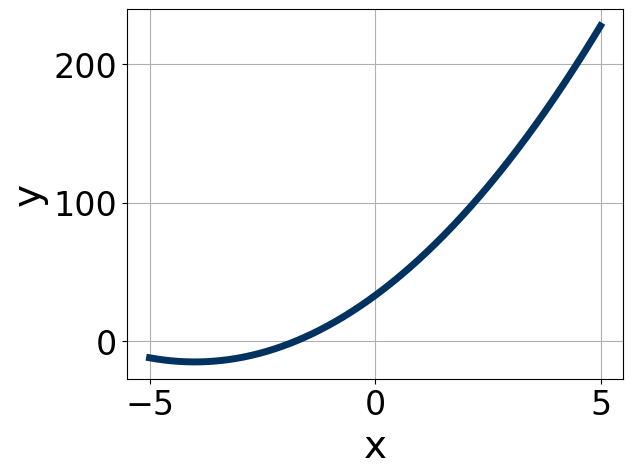
\includegraphics[width = 0.3\textwidth]{../Figures/quadraticEquationToGraphAB.png}\item 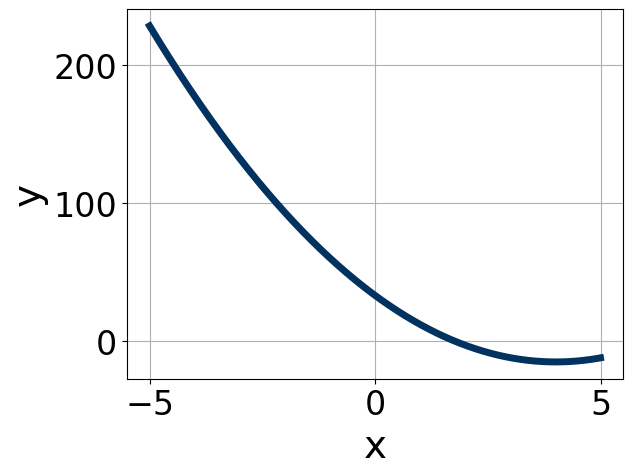
\includegraphics[width = 0.3\textwidth]{../Figures/quadraticEquationToGraphBB.png}\item 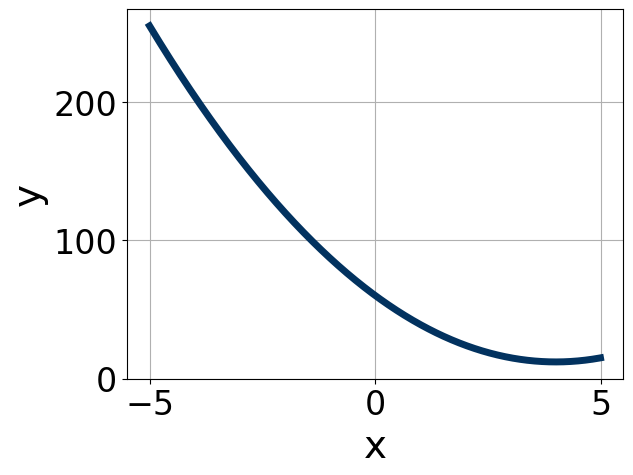
\includegraphics[width = 0.3\textwidth]{../Figures/quadraticEquationToGraphCB.png}\item 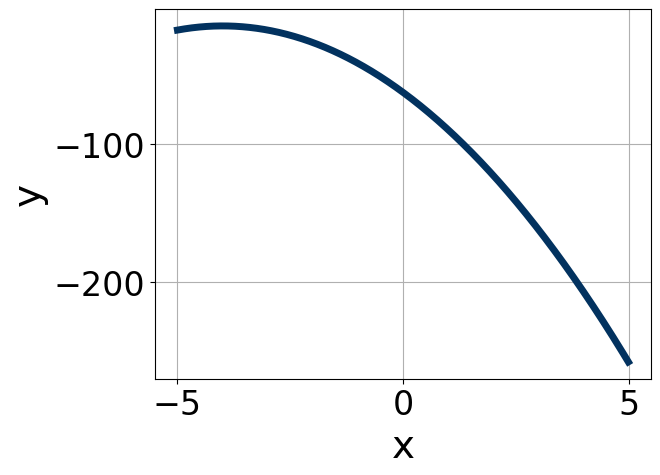
\includegraphics[width = 0.3\textwidth]{../Figures/quadraticEquationToGraphDB.png}\end{multicols}\item None of the above.
\end{enumerate} }
\litem{
Write the equation of the graph presented below in the form $f(x)=ax^2+bx+c$, assuming  $a=1$ or $a=-1$. Then, choose the intervals that $a, b,$ and $c$ belong to.
\begin{center}
    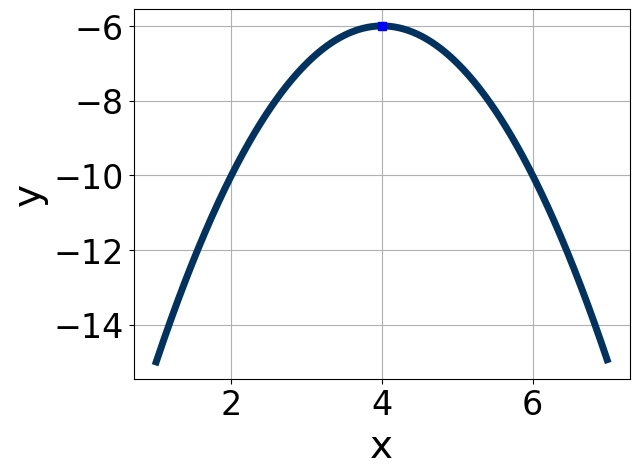
\includegraphics[width=0.5\textwidth]{../Figures/quadraticGraphToEquationCopyB.png}
\end{center}
\begin{enumerate}[label=\Alph*.]
\item \( a \in [1, 2], \hspace*{5mm} b \in [-9, -6], \text{ and } \hspace*{5mm} c \in [8, 13] \)
\item \( a \in [-1, 0], \hspace*{5mm} b \in [-9, -6], \text{ and } \hspace*{5mm} c \in [-26, -21] \)
\item \( a \in [-1, 0], \hspace*{5mm} b \in [8, 12], \text{ and } \hspace*{5mm} c \in [-8, -6] \)
\item \( a \in [1, 2], \hspace*{5mm} b \in [8, 12], \text{ and } \hspace*{5mm} c \in [8, 13] \)
\item \( a \in [-1, 0], \hspace*{5mm} b \in [8, 12], \text{ and } \hspace*{5mm} c \in [-26, -21] \)

\end{enumerate} }
\end{enumerate}

\end{document}